% Más Bueno -- More Than A Hack 2027, Phase 1 technical document.
% Build: pdflatex docs/technical_document.tex (run twice; figure: python docs/figures.py first)
\documentclass[11pt,a4paper]{article}
\usepackage[margin=2.2cm]{geometry}
\usepackage[T1]{fontenc}
\usepackage{lmodern}
\usepackage{microtype}
\DisableLigatures[-]{encoding = T1, family = tt*} % keep -- as two hyphens
\usepackage{booktabs}
\usepackage{array}
\usepackage{tabularx}
\usepackage{enumitem}
\usepackage{amsmath}
\usepackage{graphicx}
\usepackage{xcolor}
\usepackage{tikz}
\usetikzlibrary{arrows.meta,positioning,calc}
\usepackage{caption}
\usepackage{float}
\usepackage{xurl}
\usepackage{hyperref}
\hypersetup{
  colorlinks=true, linkcolor=blue!60!black, urlcolor=blue!60!black, citecolor=blue!60!black,
  pdftitle={Possession from automatic tracking: a gated three-state decoder},
  pdfauthor={Team Más Bueno: Aaron Binoj Amacadu, James Joshua Koshy, Karthik Nambiar Puthiyedathu Velluva},
  pdfsubject={More Than A Hack 2027, Phase 1 technical document}
}
\setlist{itemsep=0.15em, topsep=0.3em, parsep=0pt}
\captionsetup{font=small, labelfont=bf}
\setlength{\parskip}{0.35em}
\setlength{\parindent}{0pt}
\setlength{\emergencystretch}{2em}
\renewcommand{\arraystretch}{1.12}
\newcolumntype{P}[1]{>{\raggedright\arraybackslash}p{#1}}
\newcolumntype{L}{>{\raggedright\arraybackslash}X}
\newcommand{\code}[1]{\texttt{#1}}
\newcommand{\st}[1]{\textbf{#1}}
% neutral colours for the pipeline figure
\colorlet{ink}{black}\colorlet{muted}{black!65}\colorlet{accent}{black!70}
\colorlet{navy}{black}\colorlet{panel}{black!4}\colorlet{rule}{black!40}

\begin{document}

% ---------------------------------------------------------------- title
\begin{center}
{\LARGE Possession from automatic tracking:\\[0.25em] a gated three-state decoder\par}
\vspace{1.0em}
{\large Team Más Bueno\par}
\vspace{0.4em}
Aaron Binoj Amacadu \qquad James Joshua Koshy \qquad Karthik Nambiar Puthiyedathu Velluva\par
\vspace{0.6em}
{\small More Than A Hack 2027, Phase 1 -- technical document -- 17 November 2026\par
Code: \url{https://github.com/4139benuzter/mtah2027-mas-bueno} \par Submission file (GRU hybrid), SHA-256 \texttt{2824617531b9bcda\ldots{}fed279cac825065504}\par}
\end{center}
\vspace{0.5em}

\begin{abstract}
We label every frame as home (\code{H}), away (\code{A}) or dead ball
(\code{D}) with a three-state hidden Markov chain decoded by Viterbi. The challenge's own
definition of possession is written into the decoder: a change of side is cheap \emph{only} where
the gaining side starts a controlled contact or a completed pass; touches, deflections and duels
are neutral; the ball is dead when it is out, between going out and the restart kick, or when
nobody on the pitch is running. There is no machine-learning model trained on this match, no
label of this match was used, and the pipeline (numpy and pandas, about 15\,s on a laptop) contains
no language model. Every setting that is not a physical or football quantity was chosen on
\emph{other} labelled matches, by selection rules committed to the repository before their results
existed. The submitted file keeps this decoder's dead-ball decisions and, where the ball is
alive, takes the side from a bidirectional GRU network trained only on other matches (the GRU hybrid
of Section~3).

\end{abstract}

\begin{center}\small
\begin{tabularx}{\linewidth}{@{}Lrrrr@{}}
\st{spellF1, official scorer} & \st{Metrica (3)} & \st{DFL (7)} & \st{SkillCorner (19)} & \st{Floor} \\
\midrule
v31 (the hand-built decoder) on labelled other matches\textsuperscript{*} & 0.576 & 0.454 & 0.550 & 0.2433 \\
Submitted GRU hybrid: held-out gain over v31, degraded balls\textsuperscript{\dag} & $+0.108$ & $+0.100$ & -- & \\[-0.2em]
\multicolumn{5}{@{}l}{\footnotesize\color{muted}\textsuperscript{*}Metrica and DFL: mean over the ball as recorded and cut to the competition's 59\% visibility (Section 5).} \\[-0.3em]
\multicolumn{5}{@{}l}{\footnotesize\color{muted}\textsuperscript{\dag}Each match predicted by models trained on the other nine; the hybrid is described in Section 3.} \\
\end{tabularx}
\end{center}

% ---------------------------------------------------------------- 1
\section{Approach}

The ranking metric scores \emph{whole possessions}
(intervals matched by overlap), so the shape of the output over time matters more than any
single frame. No labels of this match may be used for training. Labels of other matches do exist,
but they disagree with each other about what a possession is (Section~5), so a classifier trained on
them would learn their conventions rather than the challenge's. The challenge, on the other hand,
states its conventions in words: possession changes when the other side gains \emph{controlled}
possession; a touch, a deflection or a duel won without control does not count; a loose ball
stays with the last side. We therefore express every cue as a per-frame log-probability of the
three states and let a Viterbi pass find the most probable sequence, with a cost charged for every
change of state. The chain changes its answer only when evidence for the new state, accumulated
over consecutive frames, outweighs that cost: this is what turns noisy frames into possessions.
The submitted file adds one learned part (Section~3): where this decoder says the ball is alive, a
bidirectional GRU network trained only on other matches chooses the side; the decoder's dead-ball
decisions are kept unchanged.

\begin{figure}[h]
\centering
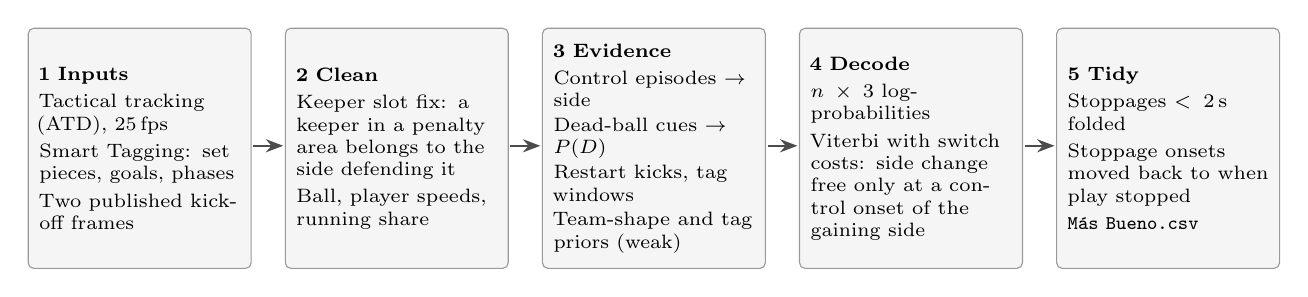
\begin{tikzpicture}[
  font=\scriptsize, node distance=0.42cm,
  box/.style={draw=rule,fill=panel,rounded corners=2pt,align=left,text width=2.55cm,
              minimum height=3.05cm,inner sep=4pt,anchor=north},
  head/.style={font=\scriptsize\bfseries\color{navy}},
  arr/.style={-{Stealth[length=2.2mm]},draw=accent,line width=0.9pt}]
\node[box] (in) {{\color{navy}\bfseries 1 Inputs}\\[2pt]Tactical tracking (ATD), 25\,fps\\[2pt]
  Smart Tagging: set pieces, goals, phases\\[2pt]Two published kick-off frames};
\node[box,right=of in] (fix) {{\color{navy}\bfseries 2 Clean}\\[2pt]Keeper slot fix: a keeper in a
  penalty area belongs to the side defending it\\[2pt]Ball, player speeds, running share};
\node[box,right=of fix] (ev) {{\color{navy}\bfseries 3 Evidence}\\[2pt]Control episodes $\rightarrow$
  side\\[1pt]Dead-ball cues $\rightarrow P(D)$\\[1pt]Restart kicks, tag windows\\[1pt]Team-shape and
  tag priors (weak)};
\node[box,right=of ev] (dec) {{\color{navy}\bfseries 4 Decode}\\[2pt]$n\times3$ log-probabilities\\[2pt]
  Viterbi with switch costs: side change free only at a control onset of the gaining side};
\node[box,right=of dec] (out) {{\color{navy}\bfseries 5 Tidy}\\[2pt]Stoppages $<2$\,s folded\\[2pt]
  Stoppage onsets moved back to when play stopped\\[2pt]\code{Más Bueno.csv}};
\draw[arr] ($(in.north east)+(0.02,-1.5)$) -- ($(fix.north west)+(-0.02,-1.5)$);
\draw[arr] ($(fix.north east)+(0.02,-1.5)$) -- ($(ev.north west)+(-0.02,-1.5)$);
\draw[arr] ($(ev.north east)+(0.02,-1.5)$) -- ($(dec.north west)+(-0.02,-1.5)$);
\draw[arr] ($(dec.north east)+(0.02,-1.5)$) -- ($(out.north west)+(-0.02,-1.5)$);
\end{tikzpicture}
\caption{The pipeline. One command (\code{python make\_submission.py}) runs all five stages.}
\end{figure}

\subsection{Who has the ball: control episodes and their outcomes}

Whether a touch was control depends on what happened next, which per-frame ``nearest player''
evidence cannot express. We cut tracked play into \emph{contact episodes}: runs of at least two
frames where the ball is within 1.5\,m of a player and moving at roughly that player's speed (a
ball flying past a player is not contact). Each episode is classified by its length and by where
the ball went next (\code{possession/episodes.py}):

\begin{center}\small
\begin{tabularx}{\linewidth}{@{}l L l@{}}
\toprule
\st{Episode} & \st{Definition} & \st{Evidence} \\
\midrule
controlled & contact of at least 0.6\,s moving with the player, whatever follows & strong, for that side \\
pass & shorter contact whose next contact is a team-mate within 4\,s & strong, over contact and flight \\
touch & contact under 0.6\,s whose next contact is an opponent & none \\
unresolved & contact under 0.6\,s followed by a lost ball or nothing for 4\,s & none \\
\bottomrule
\end{tabularx}
\end{center}

The 0.6\,s \emph{carry rule} follows from physics: a deflection or block leaves a player at well
over 3\,m/s and crosses the 3\,m contact disc in well under a second, so a ball that stays with the
player longer was received or carried. Touches and unresolved contacts are \emph{neutral}, not
evidence for the other side, exactly as the challenge says. A down-weighted per-frame contact term
(log-odds weight 0.5, muted to 0.1 inside touches and 0.3 inside unresolved contacts) lets
sustained but untidy contact count without letting a touch accumulate into a change of side. A
kick out of a stoppage credits the kicker's side for 0.8\,s, and Smart Tagging transition tags
credit the gaining side for 3\,s at 0.5 nats per frame.

\subsection{Dead ball}

Several cues set the dead-ball probability of each frame: the ball tracked more than 0.3\,m outside
the pitch ($P(D)=0.9$); \emph{nobody running} --- the share of players above 2\,m/s is bimodal over
the match, and a threshold of 0.05 in its trough separates 70\% of dead frames from 84\% of alive
ones (measured against tagged set-piece and build-up windows, not labels), mapped by a logistic
ramp to $P(D)$ between 0.12 and 0.60; a ball at rest for about 2\,s, or slow and ignored by everyone
($\geq0.6$); a ball walked along a line ($\geq0.55$, a throw-in or goal kick being set up); and a
\emph{restart hold} from the moment the ball goes out until a kick from a player's feet that play
actually follows ($\geq0.5$). Smart Tagging adds hard windows: the 15\,s before the detected restart
of each set-piece tag are dead and the 0.8\,s after it favour the restarting side; a goal is dead
from the start of the longest quiet stretch before the kick-off tag until the kick-off. No tag
window may force a dead ball on a frame that visibly shows play (ball moving above 3\,m/s with
more than a tenth of the players running).

\subsection{Goalkeepers, and the lost ball}

The tracker keeps one keeper slot per team, and the two keepers sometimes swap slots: the away
slot sits inside the \emph{home} penalty area on 9\% of its first-half and 13\% of its second-half
frames. A keeper holding the ball then reads as the other side, producing whole false
possessions. \code{possession/keepers.py} applies a football rule before any feature is
computed: a goalkeeper inside a penalty area belongs to the side defending that goal (15,945 frames
of the away slot and 1,501 of the home slot are re-teamed; no label is involved).

The ball is missing on 41\% of graded frames, in long stretches (median 11\,s). Three quarters of
those frames have nobody running and are stoppages, which the running-share cue handles. Elsewhere
the chain carries its last state, nudged by two deliberately weak priors: the lateral spread of
each team (the side in possession plays wider; one logistic slope fitted to pseudo-labels the
tracking itself produces where the ball is unambiguously at one side's feet, 84\% agreement on
29,234 frames) and the Smart Tagging phase team (0.05 nats per frame).

\subsection{Decoding}

Entering or leaving \code{D} costs 25 nats. A change of side costs 15 nats \emph{except within
$\pm0.2$\,s of the onset of a controlled or pass episode of the side gaining the ball, where it is
free}. This gating is the challenge's definition written into the decoder: with one fixed cost
everywhere, a short possession inside the other side's play would need two full switches and be
overruled however clean the control was. Two post-passes follow: dead-ball spells shorter than
2\,s are folded into the next spell (a stoppage cannot be that short), and each stoppage onset is
moved back to the moment the running share began to fall, because the decoder places the boundary
where evidence tips, a second or two after the whistle.

% ---------------------------------------------------------------- 2
\section{Assets used, and dropped}

\begin{center}\small
\begin{tabularx}{\linewidth}{@{}l L l@{}}
\toprule
\st{Asset} & \st{How it is used} & \st{Status} \\
\midrule
Tactical ATD & the only positional evidence; keeper slots corrected (Section 1.3) & \textbf{used} \\
Smart Tagging & set pieces and goals as dead-ball windows; phase teams as a weak prior. Phases are not
possessions: 36 instances carry no team, every throw-in among them & \textbf{used} \\
Homography & not needed (tracking is already in pitch metres); used only to draw tracking over video when debugging & inspection only \\
Broadcast ATD & aligned to the tactical clock by matching player positions (constant offsets of
+4,014 and +26,920 frames per half; 39\% of frames within 1\,m). As a ball gap-filler it covers
only 1.8\% of graded frames and improved no check & dropped \\
Video & no labels from video; no GPU, and the hard part is the semantics of control, not detection.
Watched through our clip renderer to debug (how the keeper swaps were found) & inspection only \\
\bottomrule
\end{tabularx}
\end{center}

% ---------------------------------------------------------------- 3
\section{Training data, validation data, and the public window}

No label of this match was used, and nobody labelled any data by hand. The decoder has a single fitted number,
the team-shape slope, fitted to the tracking's own pseudo-labels. Labelled data of \emph{other}
matches was used to measure versions, to choose or re-examine settings, and to train the side
models of the hybrids (LightGBM for the first, a bidirectional GRU for the submitted one; the 3 Metrica and 7 DFL matches with balls degraded to
this match's statistics, every 10th graded frame, each also with the teams swapped; Section 3):

\begin{center}\small
\begin{tabularx}{\linewidth}{@{}P{2.75cm} P{1.75cm} L P{3.3cm}@{}}
\toprule
\st{Dataset} & \st{Matches (possessions)} & \st{Labels: source and producer} & \st{Used for} \\
\midrule
Metrica sample matches 1--3\newline{\footnotesize\color{muted}\url{github.com/metrica-sports/sample-data}} & 3 (1,150) &
Metrica's human event data, turned into frames with the competition definition by
\code{possession/sample\_game.py} (owner changes only at an event in which a player plays the ball) &
training the side models; measuring versions; choosing v31's settings; re-examining constants \\
DFL / Sportec open data\newline{\footnotesize\color{muted}Bassek et al.\ 2025, \emph{Sci.\ Data}, CC BY 4.0} & 7 (3,061) &
the per-frame \code{BallPossession} and \code{BallStatus} of official DFL position data
(\code{possession/dfl.py}): the same kind of source as the competition ground truth & the same \\
SkillCorner open data\newline{\footnotesize\color{muted}\url{github.com/SkillCorner/opendata}, MIT} & 19 tested + 1 (5,146) &
SkillCorner's automatic possession and interruption events, turned into frames by
\code{possession/skillcorner.py} & independent check; last selection round \\
\bottomrule
\end{tabularx}
\end{center}

Because the competition ball is visible on only 59\% of graded frames, each Metrica and DFL match is
also scored with the ball removed in random 0.4--5\,s gaps down to 59\% (two seeds). Smart Tagging
does not exist for these matches and their player identities are fixed, so those terms and the keeper
fix are off there (\code{possession/validate.py}).

Every choice below followed the same protocol, written to the
repository \emph{before} the corresponding jobs ran: score each candidate setting on each match by
its spellF1 averaged over ball conditions; pick, among settings within 0.003 of the best mean, the
one that changes the fewest values; estimate the gain honestly by leaving each match out in turn
(pick on the others, score on the one left out); adopt only if that held-out gain clears a fixed
bar, is positive in every group, and the competition match still passes label-free checks.

\begin{itemize}
\item \st{v31} (\code{calib/grid\_rule.md}): 648 combinations of seven existing settings on Metrica and
DFL. All ten held-out picks were identical: carry time 1.0\,$\rightarrow$\,0.6\,s and minimum contact
3\,$\rightarrow$\,2 frames. Held-out gain $+0.020$ (Metrica $+0.023$, DFL $+0.019$), positive on all ten
matches (smallest $+0.011$); a bootstrap over matches gave $+0.019$ (5th percentile $+0.012$).
\item \st{Re-examination} (\code{calib/grid\_window\_rule.md}): 576 combinations of the constants
first set during development (below). Best held-out gain $+0.002$ against a bar of $+0.010$: values kept.
\item \st{Independent check} (\code{calib/skillcorner\_rule.md}): on SkillCorner v31 is $0.021$ below v30
(95\% interval $-0.026$ to $-0.016$). The rule then re-ran the selection with three equally weighted
groups; its pick was v31 itself. Section~5 explains the conflict.
\item \st{New logic, round 1} (\code{calib/v32\_rule.md}): 162 combinations of four new rules
(dead-ball probability when the ball is lost; folding short same-side stoppages; folding sub-second
possessions inside the other side's play or just before a stoppage), on Metrica and SkillCorner.
The pick (fold possessions under 1\,s inside the other side's play) was the same in all 22 folds and
helped 21 of 22 matches, but its held-out gain was $+0.0092$ against a bar of $+0.010$. \textbf{v31
was kept.} Lowering the dead-ball probability when the ball is lost hurt in both groups.
\item \st{New logic, round 2: the lost ball} (\code{calib/v33\_rule.md}): straight-line filling of ball gaps up to 0.5--2\,s, and moving a change of side that follows a ball gap to the middle of the gap (12 combinations, ball as recorded only, since the artificial gaps are far shorter than the competition's real ones). Every held-out pick was v31 itself and no combination moved the mean by more than 0.0012: \textbf{v31 was kept.}
\item \st{New logic, round 3: ideas from other teams} (\code{calib/v34\_rule.md}): on the last evening we read the code and documentation (never data or results) of other teams' public repositories and re-implemented three ideas our decoder lacked: starting a stoppage where the ball is seen leaving the pitch, ignoring out-of-pitch sightings that are back in play within 1\,s (aerial balls), and moving a change of side back to the new side's first contact (12 combinations). Every held-out pick was v31 itself; the best combination moved the mean by $+0.0009$, and the exit snap helped Metrica ($+0.003$) but cost SkillCorner ($-0.009$). \textbf{v31 was kept.}
\item \st{Learned evidence, a parallel series, not submitted} (branch \code{touch-detector}; files \code{calib/touch\_*},
\code{domain\_*}, \code{learned\_*}, where the attempts are called v32--v35c, a separate series from the rounds
above). Six attempts, each with a rule committed before its result, on the Metrica and DFL matches with their
balls degraded to match 17 label-free statistics of this match's ball (\code{calib/domain\_target.json}) and
SkillCorner as a check. The strongest, a LightGBM frame classifier decoded by v31's own decoder (v35c), gained
$+0.119$ held out (10 of 10 matches; SkillCorner $+0.008$) but failed our transfer check: on this match it gave
22\% more possessions than v31 (346 against 284), against at most 6\% on the public matches, so the rule kept
v31. On 17 November at about 23:50 (UTC+4) the team overrode that rule and pushed v35c to the repository for
the rank objective (\code{calib/learned\_c\_override.md}). At about 01:25 the frozen v35c file was scored once
on the public window, for information: macroF1 0.7027, spellF1 0.4121 (Section~5); it called a 20\,s
stoppage alive. The team then returned to v31, the version the pre-committed rule had kept and the file
submitted since 16 November, before the deadline. \textbf{This last decision came after that window score,} and
we disclose it as such; nothing was tuned on the window, and no setting of v31 changed.
\item \st{The first hybrid} (\code{calib/hybrid\_rule.md}, committed at 02:14 UTC+4 before any
hybrid number). Dead ball from v31; where v31 says the ball is alive, the side from v35c where v35c says
home or away, otherwise v31's side. Held out on the ten public matches it gained $+0.034$ spellF1 over v31
(10 of 10 matches; Metrica $+0.040$, DFL $+0.031$) and about $+0.01$ macroF1; on this match it gives 285
possessions (v31: 284) and v31's dead-ball checks (Section~5). It passed every condition of its rule. The idea came after v35c's window score showed weak dead-ball timing; we disclose
that. The hybrid itself was never scored on the window.
\item \st{The submitted GRU hybrid} (\code{calib/gru\_rule.md}). Before any result (about 02:37 UTC+4, stated
in the team's chat, committed with the result) the rule was: a held-out gain of at least $+0.010$ over the first
hybrid, on at least 8 of the 10 matches, positive for Metrica and for DFL. A bidirectional GRU (two layers of 64
units over 30\,s windows of the same 67 features, trained on the same degraded matches with the teams
swapped) replaces the trees for the side; the dead ball stays v31's. Held out on the ten public matches it scored
0.564 against 0.495 for the first hybrid ($+0.069$, 10 of 10; v31 0.462), and on this match it gives 293
possessions (v31: 284), v31's dead-ball checks and 80.2\% side agreement. It runs in numpy from
\code{calib/gru\_model.npz} (equal to PyTorch within $2\times10^{-7}$). The GRU alone scored 0.656 held out
but was not used: its own dead-ball calls carry the risk that v35c showed on this match. It was built and
tested in the last hour before the deadline. After it was frozen and pushed, the submitted file was scored once on
the window at the team's request, for information only (Section~5); the score did not change it.
\end{itemize}

The public 5-minute window was used to confirm alignment and file format and
to debug \emph{mechanisms} (how the one-second carries and the swapped keeper slots were found). But
during development versions v24--v27 were also scored on it, and four choices were made with it in
view: neutral weight for touches and unresolved contacts; a 3-frame minimum pass contact; the
stoppage-onset pass and its constants; and very probably the 0.88 strength of controlled and pass
evidence. An earlier draft said the window set no number; that was not accurate. From v28 on no
version was chosen with it (with one exception on the last night, the return
from v35c to v31 and the hybrid that followed, disclosed above), the tools no longer read it by default, the minimum contact was replaced
by a value chosen on other matches, and the other constants were re-examined on other matches (the
re-examination above): none of the alternatives passed, and each moved the mean by at most 0.002.
The final version was frozen before it was scored on the window; it was scored once afterwards, for
information only (Section~5).

% ---------------------------------------------------------------- 4
\section{Possession rules implemented}

\begin{center}\small
\begin{tabularx}{\linewidth}{@{}P{3.7cm} L@{}}
\toprule
\st{Situation} & \st{Our rule} \\
\midrule
Change of possession & only where the other side starts a controlled contact ($\geq0.6$\,s with the
player) or a completed pass; the decoder makes the switch cheap only there \\
Touch, block, deflection & neutral evidence: a contact under 0.6\,s that goes to an opponent, or to
nobody, does not change possession \\
Aerial duel, challenge & neutral unless the winner's side then controls the ball or completes a pass \\
Loose or contested ball & stays with the last side in possession (the chain holds its state) \\
Ball not tracked & the last state is held; weak team-shape and tag priors only break long silences \\
Goalkeeper & a keeper inside a penalty area belongs to the side defending it \\
Ball out, foul, offside & dead from the stoppage until the restart kick that play follows; the onset
is moved back to when the players stopped \\
Restart (throw-in, goal kick, free kick, corner, kick-off) & begins a possession for the restarting
side, credited for 0.8\,s after the kick, then normal evidence \\
Goal & dead from the goal (start of the longest quiet stretch before the kick-off tag) to the kick-off \\
\bottomrule
\end{tabularx}
\end{center}

% ---------------------------------------------------------------- 5
\section{Results}

On labelled other matches (official \code{evaluation/possession\_metrics.py}, spellF1). v31's two
settings were chosen on Metrica and DFL, so those columns are in-sample; its held-out gain over v30
is $+0.020$ (Section~3).

\begin{center}\small
\begin{tabular}{@{}l l r r r r@{}}
\toprule
\st{Group} & \st{Ball} & \st{v30} & \st{v31} & \st{Possessions: labels} & \st{v31} \\
\midrule
Metrica (3) & as recorded & 0.565 & \textbf{0.587} & 383 & 262 \\
Metrica (3) & cut to 59\% & 0.547 & \textbf{0.570} & 383 & 254 \\
DFL (7) & as recorded (100\%) & 0.521 & \textbf{0.544} & 437 & 282 \\
DFL (7) & cut to 59\% & 0.392 & \textbf{0.409} & 437 & 234 \\
SkillCorner (19) & as recorded ($\approx$55\%) & \textbf{0.570} & 0.550 & 256 & 329 \\
\bottomrule
\end{tabular}
\end{center}

\begin{figure}[h]
\centering
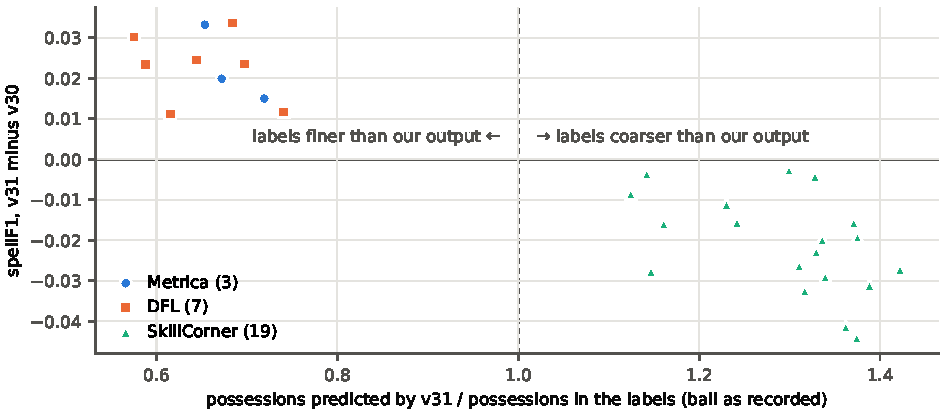
\includegraphics[width=0.93\linewidth]{fig_granularity.pdf}
\caption{Why the groups disagree. Each point is one match (ball as recorded). Where the labels
count \emph{more} possessions than we output (Metrica, DFL), v31 beats v30 on every match; where they
count fewer (SkillCorner, whose labels only change owner at clean, algorithm-detected possessions),
v31 loses on every match. The sign of a change follows the granularity of the labels, and the
granularity of the competition's labels is unknown; we did not, and may not, estimate it from the
public window. By source, the DFL labels are closest to the competition's: per-frame possession and
ball-status fields of official position data.}
\end{figure}

On the competition match, without labels (\code{possession/diagnose.py}; Smart Tagging and
tracking only):

\begin{center}\small
\begin{tabular}{@{}l r r r@{}}
\toprule
\st{Check} & \st{v27} & \st{v30} & \st{v31} \\
\midrule
possessions (mean length) & 209 (15.9\,s) & 242 (13.8\,s) & 284 (11.8\,s) \\
possessions shorter than 2\,s & 7\% & 13\% & 16\% \\
graded frames dead & 47.7\% & 47.5\% & 47.5\% \\
dead inside tagged build-up, progression and transition phases & 9.2\% & 8.7\% & 8.7\% \\
dead inside the 3\,s before a tagged set piece & 94.5\% & 94.6\% & 94.6\% \\
same side as a tagged phase, where we say the ball is alive & 84.2\% & 83.3\% & 82.2\% \\
\bottomrule
\end{tabular}
\end{center}

The submitted hybrid gives 285 possessions (11.7\,s), 12\% shorter than 2\,s, 47.5\% dead, 8.7\% and
94.6\% on the two dead-ball checks, and 80.4\% side agreement. Home share of alive time is 63\% for v31. Phases are not possessions (a phase can outlast several changes of
side), so the side agreement is a sanity bound, not a target; the official baseline scores 67\% on it.

On the public window, for information only (17 true possessions; never used to choose v31; the idea of the submitted hybrid came after the v35c score,
Section~3):

\begin{center}\small
\begin{tabular}{@{}l r r r@{}}
\toprule
\st{Submission} & \st{macroF1} & \st{spellF1} & \st{Possessions} \\
\midrule
\code{baseline\_smooth50} (official floor) & 0.6207 & 0.3256 & 26 \\
ours, v27 & 0.9010 & 0.5143 & 11 \\
ours, v30 & 0.9089 & 0.5286 & 11 \\
ours, v31 (not submitted; scored after it was frozen) & 0.9021 & 0.5375 & 15 \\
ours, GRU hybrid (submitted; scored once after it was frozen and pushed) & 0.9267 & 0.6069 & 12 \\
ours, v35c (not submitted; scored once, Section~3) & 0.7027 & 0.4121 & 16 \\
\bottomrule
\end{tabular}
\end{center}

With 17 possessions the segment-bootstrap intervals of our versions overlap almost entirely (about
0.31 to 0.72), so the window cannot rank them; the other matches above are the better guide.

% ---------------------------------------------------------------- 6
\section{Limitations, and what we would do with more time}

\begin{itemize}
\item The side model of the submitted hybrid (a BiGRU, built in the last hour) was trained on Bundesliga and Metrica matches whose
balls were degraded to this match's statistics; the players' tracking was not degraded, and its running-share
input divides by all player slots (48 here, 26--40 in training). It improved every public match, but its effect
on this match could not be measured. \emph{Next:} degrade the players too, and train a sequence model.
\item The lost ball is the largest loss. On DFL, removing the ball down to the competition's 59\%
visibility lowers v31 from 0.544 to 0.409. When the ball is missing we only hold the last state; filling short gaps with a straight line and placing hand-overs inside gaps changed nothing on other matches (Section~3), because the missing information is not in the tracking.
\emph{Next:} a ball-carrier model learned from other matches' tracking (who is pressed, where the
team is running), and the aligned broadcast feed as a second ball observer.
\item With the ball as recorded, v31 outputs 58--74\% as many possessions as
the DFL labels contain; possessions under about 2\,s are mostly missed, often because the tracking
shows no control episode at all (one brief touch, or no ball).
\item The best setting depends on how finely the ground truth
counts possessions (label granularity, Figure~2), which we could not measure without breaking the rules. \emph{Next:} labels of the
same kind as the competition's (corrected tracking) for calibration, and a segment-level decoder
that optimises the overlap-based metric directly.
\item Boundaries are placed to within about a second, not to the frame; possessions that begin
with an untidy recovery are often credited late.
\item Goalkeepers are often absent from the tracking (a keeper holding the ball then looks like a
slow ball nobody is near), and the slot correction applies only inside the penalty areas.
\item The tracked ball trails the video by about three frames (measured label-free); the
ground truth runs on the tracker's clock, so no correction is applied for scoring.
\item Other matches are scored without Smart Tagging and without the keeper
fix, on labels that are not Metrica's corrected tracking. They show the direction and size of a
change, not the competition score.
\end{itemize}

% ---------------------------------------------------------------- 7
\section{Reproduction}

\begin{quote}\small\ttfamily
pip install -r requirements-possession.txt\hfill\textrm{\color{muted}\# Python 3.12 or newer}\\
python make\_submission.py --team "Más Bueno"\hfill\textrm{\color{muted}\# about 15\,s, deterministic}\\
python evaluation/validate\_submission.py "evaluation/results/Más Bueno.csv"
\end{quote}

Data go in \code{./data} as described in \code{DATA.md} (or \code{MTAH\_DATA\_DIR}). The run is
deterministic: the same data give a byte-identical file (the GRU hybrid, \code{gru\_hybrid = True} in \code{possession/model.py}), with SHA-256\\
{\small\texttt{2824617531b9bcda2e2be323294df14c631589fe21ff40fed279cac825065504}}; with both switches off the same command gives v31's file\\
{\small\texttt{f34036f02e246b42f314e1de70d7d6b1cc15aca906d65a686d6963a32604de2a}}. v31's file was reproduced on two machines and with two numpy/pandas versions (pinned numpy
2.5.0 / pandas 3.0.3, and 2.3.5 / 3.0.0); the hybrid's file was regenerated from a fresh clone with the pinned
versions. The classifier runs from the committed trees in \code{calib/learned\_model.json} with numpy
only, and the BiGRU from \code{calib/gru\_model.npz} with numpy only (\code{possession/gru.py}); re-training
needs \code{requirements-train.txt} (LightGBM 4.7.0, PyTorch 2.11 with CUDA), \code{hpc/learned.pbs} and
\code{calib/gru\_train.py}; the BiGRU's held-out test is \code{calib/gru\_lomo.py} with output in
\code{calib/gru\_lomo\_output.txt}. The
held-out test of the hybrid is \code{calib/hybrid\_test.py}, with its output in \code{calib/hybrid\_test\_output.txt}.

The validation is reproducible from public data only. \code{possession/validate.py} scores the current
decoder on one match; \code{possession/grid.py} with \code{grid\_select.py}, \code{three\_group.py} and
\code{sc\_check.py} repeat the selections of Section~3 (Linux; the DFL conversion needs kloppy 3.19.1);
\code{possession/bench.py} with \code{select\_v32.py}, and \code{bench\_v33.py} with \code{select\_v33.py}, and \code{bench\_v34.py} with \code{select\_v34.py}, repeat the three rounds of new logic (Windows or Linux). Every
result file is committed under \code{calib/}, and \code{python docs/figures.py} redraws Figure~2 from them.

% ---------------------------------------------------------------- 8
\section{Tools}

The code was written with the help of an LLM coding assistant (Claude Code, by Anthropic). Its
program runs on our machine but its language model runs on Anthropic's servers, so what it reads is
sent there. We did not give it the match data files, the video, or extracts of them: it saw file and
folder names and the summary output our scripts print (counts, shares and scores). That output
included the 17 aggregate statistics of this match's tracking in \code{calib/domain\_target.json} and
a summary of its missing ball frames (shares and rates, no frame indices); sub-agents of the same
assistant used those numbers to fit the degradation of the public balls (Section~3) and otherwise
worked on public data only. Training runs on public data used a university computing cluster; the
competition data stayed on our own machine. It also read the
public material: this repository, including the public 5-minute ground truth, and the public data of
other matches (Section~3). The submitted pipeline contains no language model and calls no service.

\end{document}
